\section{Evaluation of Environmental Wireless Sensor Networks (E-WSN)}
\label{section:experimental}	

To define our simulation clearly we will base it on a realistic deployment scenario as covered by Gomez et al \cite{Gomez} and others \cite{Jha2016, Avram}. We will use a UAV to deploy a large number of sensors over a large and remote geographical area, leading to a relatively ad-hoc, randomised placement of devices. They will use solar power cells to maintain enough energy to power themselves over a number of years, making clear the requirement for low power usage. Noting that the transceiver is the significant power drain on these sensors we can see that reducing its utilisation will be one of the keys to managing energy usage. We will design our sensors to use \textit{Wake Up Radio} (WUR) and aim our agent deployment strategy towards minimising its use and range. As mentioned, the other main driver of the way we use the agents to control the sensors will be the resilience and adaptivity of the system over long periods of time, with no human intervention possible. 

We make the following assumptions and simplifications.
\begin{itemize}{
		\item Node deployment is randomly distributed across the grid following the uniform distribution or a radial normal distribution.
		\item Energy harvesting works continuously at constant rate. This assumes consistent solar exposure and limits the simulation to daytime.
		\item Permanent node failure is based on the total energy consumption of that node over time, as a proxy for wear.
		\item Temporary loss of availability of nodes is random and at a constant rate.
	}
\end{itemize}

Example values in \ref{table:components_energy_usage} show the energy and time costs of varios operations given an hourly sampling period for a node.


\begin{table}[h]
	\begin{tabular}{p{0.3\textwidth}p{0.2\textwidth} p{0.2\textwidth} p{0.2\textwidth}}
		\hline
		Function & power(mW) & time (s) & energy (mJ)\\
		\hline
		Data acquisition (\symbolDataAcquisition{}{}) & 0.5 & 60 & 30 \\
		Transmission (\symbolTransmission{}{}) & 7 & 0.1 & 0.7 \\
		Receiver (\symbolReceiver{}{}) & 70 & 0.1 & 0.7 \\
		Idle wake-up-radio (\symbolWakeUpRadio{}{}) & 0.07 & 3509 & 246  \\
	\end{tabular}
	\caption{Component types and energy usage}
	\label{table:components_energy_usage}
\end{table}

\todo[inline]{Describe the comparison of network task layouts}
\begin{figure}[ht]
	\centering
	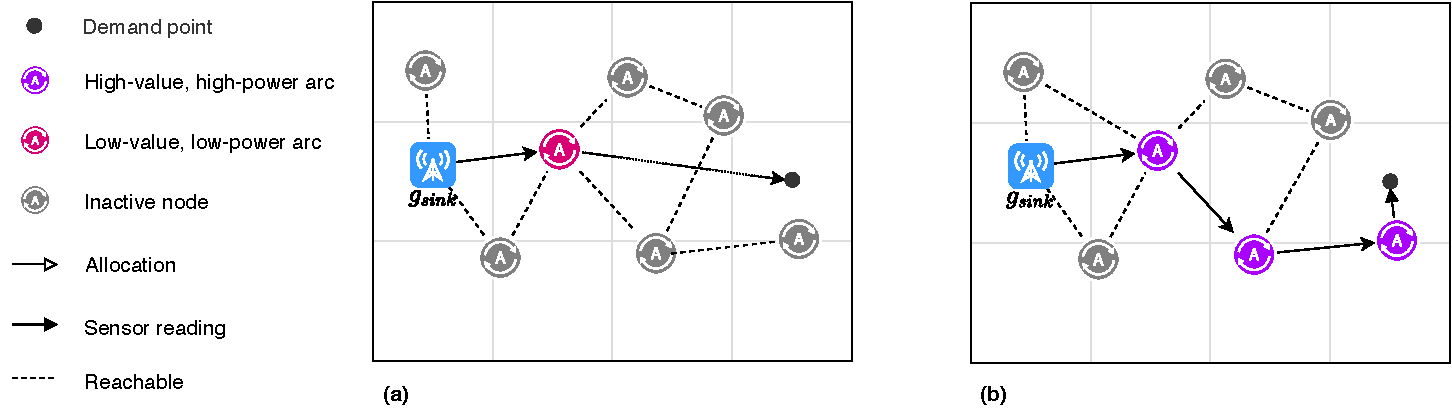
\includegraphics[width=0.9\linewidth]{network-types}
	\caption{\textbf{Experimental network type}. The diagram shows two arcs possible for the system. In arc A, the maximum quality for the task is achieved, however, there is more energy usage overall. In arc B, energy is conserved but the task is completed to a lesser quality}
	\label{fig:network-types}
\end{figure}

